El mundo de la robótica da acceso a resolver una gran variedad de problemas donde el ser humano estaba
limitado físicamente: levantar cargas de gran peso, realizar tareas repetitivas durante tiempos
prolongados, etc. Además, como bien se sabe, ha permitido el desarrollo de cadenas de producción en
masa para poder desarrollar y crear los productos que usamos diariamente, desde el coche hasta el 
teléfono móvil.

Desde que se empezó a investigar en este campo, el desarrollo de los brazos robóticos ha sido 
exponencial: se empezó trabajando con pequeños autómatas hasta el desarrollo de la revolución
industrial \cite{moran_evolution_2007}.

Los primeros modelos, como se puede ver en la figura \ref{fig:evolution}, empezaron intentando hacer
representaciones de las manos humanas. En particular, se crearon un flautista y un tamborilero los
cuales eran capaces de tocar los respectivos instrumentos utilizando un complejo sistema de cables y 
engranajes para poder mover los ``dedos'' de los músicos.

\begin{figure}[H]
    \centering
    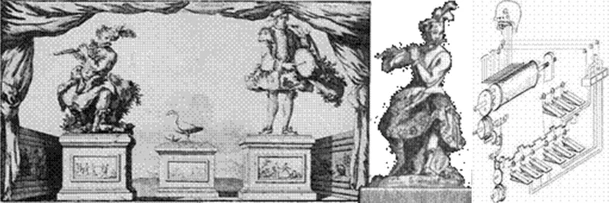
\includegraphics[width=.75\linewidth]{pictures/evolution_of_robotic_arms.png}
    \caption{Flautista y tamborilero de Vaucanson \cite{vaucanson_mecanisme_1738}.}
    \label{fig:evolution}
\end{figure}

Siguiendo con esta idea, se fue mejorando y desarrollando el modelo de imitación de las articulaciones
y los miembros de los humanos, llegando a construir estructuras más complejas y avanzadas, pensadas en 
su momento para poder tocar el clavicordio mediante un muñeco, como se muestra en la figura 
\ref{fig:lady_musician}:

\begin{figure}[H]
    \centering
    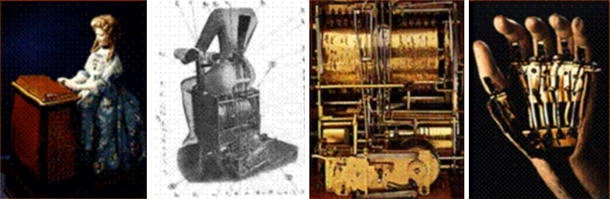
\includegraphics[width=.8\linewidth]{pictures/reproduction_of_lady_musician.png}
    \caption{En 1774, ``lady musician'' por Jaquet-Droz \cite{chapuis_alfred_and_droz_edmond_automata_1958}.}
    \label{fig:lady_musician}
\end{figure}

Durante los años siguientes, el proceso se fue refinando hasta el punto de desarrollar un autómata
el cual era capaz de jugar al ajedrez, llamado ``The Turk'' \cite{standage_tom_turk_2002}, construido
en 1769. La estructura comprendía un conjunto de mecanismos los cuales eran controlados por un operador,
encargado de realizar los movimientos del brazo izquierdo del autómata.

En la figura \ref{fig:turk} se puede ver cómo está diseñado el sistema para mover un controlador 
pantográfico sobre el tablero de juego, controlado por el operador externo antes mencionado:

\begin{figure}[H]
    \centering
    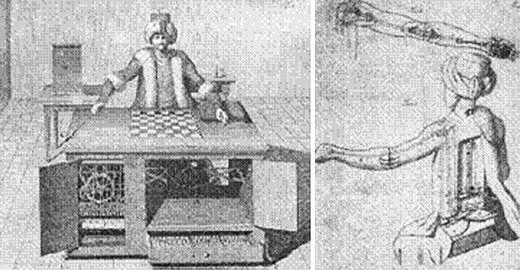
\includegraphics[width=.75\linewidth]{pictures/chess_evolution.png}
    \caption{``The Turk'', creado por von Kempelen en 1769 \cite{standage_tom_turk_2002}.}
    \label{fig:turk}
\end{figure}
